\section{Evaluation}

We now evaluate the CWMR method, our revised ASAD-CWMR, and Anticor method by performing back tests on real historical data from stock markets. The historical stock data were downloaded from Yahoo Finance. The datasets we used for backtesting are summarized in Table~\ref{tab:dataset}. Datasets NYSE-O and NYSE-N were also used in the previous works\cite{OnlinePortfolio, AntiCor}, while the up-to-date datasets NYSE-5018 and NASDAQ-5018 were collected by us.

\begin{table}
\caption{Summary of 4 real datasets from NYSE and NASDAQ.}
\label{tab:dataset}
\begin{center}
\begin{tabular}{cccc}
\hline
Dataset &  \# Stocks & Time frame &  \# Days \\
\hline
NYSE-O & 36 & July 3, 1962 -- Dec 31, 1984 & 5651 \\
NYSE-N & 23 & Jan 1, 1985 -- June 30, 2010 & 6431 \\
NYSE-5018 & 334 & Jan 1, 1995 -- Dec 5, 2014 & 5018 \\
NASDAQ-5018 & 101 & Jan 1, 1995 -- Dec 5, 2014 & 5018 \\
\hline
\end{tabular}
\end{center}
\end{table}

We set the CWMR parameters $\epsilon$ to -0.5 and $\phi$ to 2, and Anticor window size $w$ to 40. We first successfully reproduced the results of applying CWMR and Anticor on NYSE-O and NYSE-N. In FIG.~\ref{fig:old_data_chart}(a) we present a cumulative return of around $10^{18}$\% after 5600 trading days with 36 NYSE stocks in dataset NYSE-O. The cumulative return with CWMR is around  $10^{15}$ larger than if we simply follows the market. Our ASAD-CWMR method seems to be only slightly better than CWMR, but don't forget that we can save a huge amount of money by reducing the transaction cost. Both CWMR and ASAD-CWMR outperform Anticor, and we believe the reason is the correlation employed in CWMR (current day's performance and next day's performance) is much stronger than the correlation in Anticor (stock behavior in the recent $2w$ days and its performance in the next day). The results on NYSE-N (FIG.~\ref{fig:old_data_chart}(b)) also illustrate the power of CWMR and ASAD-CWMR. We may notice that none of these methods work well after the financial crisis (since the point of 5500 trading days in FIG.~\ref{fig:old_data_chart}(b)).

To further investigate the reliability and stability of CWMR and ASAD-CWMR, we tested them on the up-to-date dataset NYSE-5018 and NASDAQ-5018 which were collected by ourselves. CWMR and ASAD-CWMR did not disappoint us, and still produce an astronomical return of at least $10^{14}$\% in 5018 trading days, or 20 years in both NYSE and NASDAQ markets (FIG.~\ref{fig:long_term_chart}). However, you may notice that the total wealth achieved reaches a peak at a point around 3000 trading days in both NYSE and NASDAQ markets, which is right before the financial crisis. During the financial crisis, the poorly-performing stocks have a large chance to keep their low performance in the next few trading days, and the pattern of mean reversion almost vanishes. Therefore, the application of any mean-reversion based strategy only results in a dramatic loss during the financial crisis. Comparing the returns in the two different markets, we also find that the cumulative return goes up slightly in NASDAQ after the financial crisis, while it does not have a sign of recovery in NYSE. We consider NASDAQ to be a healthier market because NASDAQ has more high-tech companies which are more appealing to investors in recent years.

Nevertheless, we have to admit that now all these mean-reversion methods are not as powerful as they used to be. The financial crisis cast a lingering shadow on people's lives and is still influencing the way people invest their money. However, we believe there should always exist a strong correlation in the stock market. The pattern of mean reversion behavior is just being replaced by another one that requires our further investigation. 

\begin{figure}
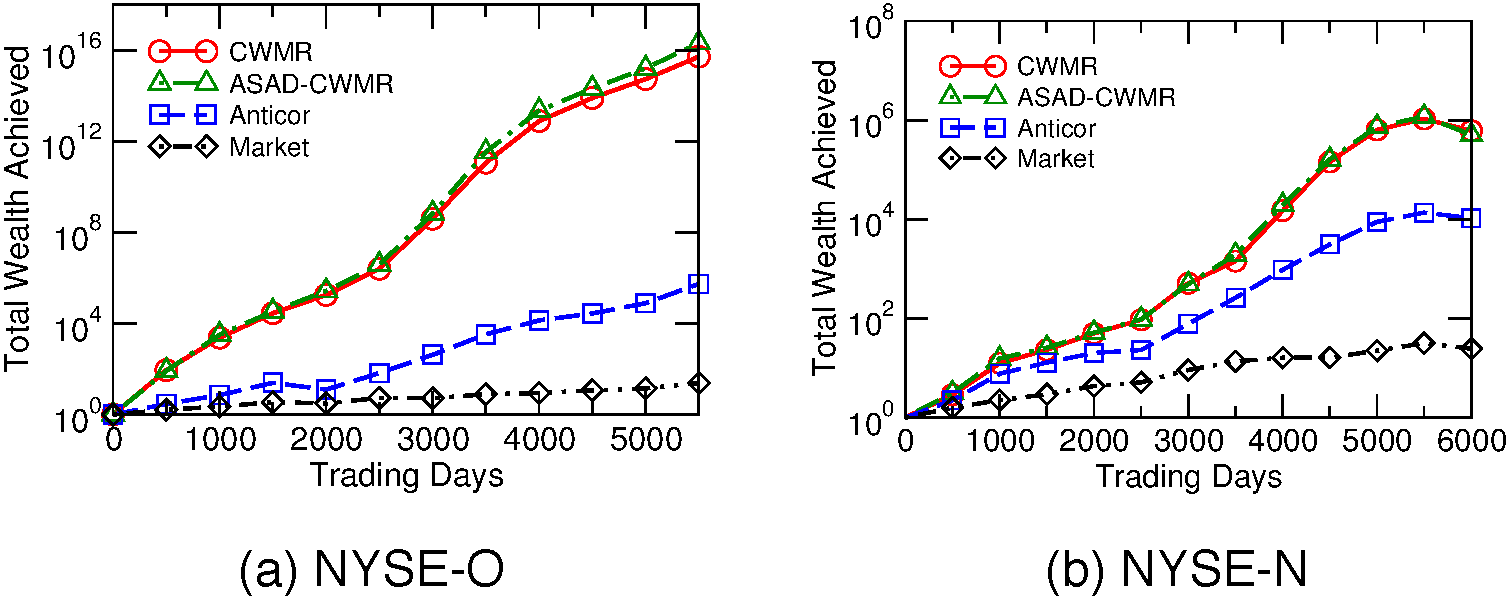
\includegraphics[width=\columnwidth]{old_data_chart}
\caption{
\label{fig:old_data_chart}
Cumulative wealth achieved in dataset (a) NYSE-O and (b) NYSE-N.
}
\end{figure}

\begin{figure}
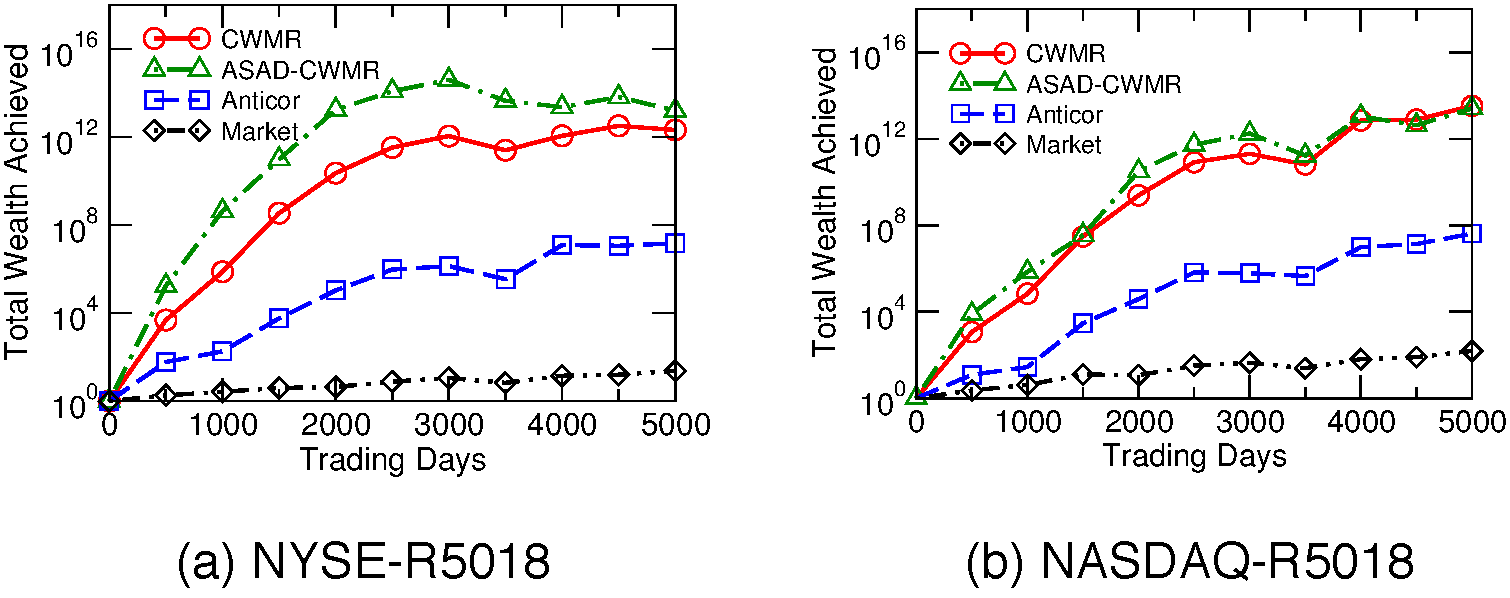
\includegraphics[width=\columnwidth]{long_term_chart}
\caption{
\label{fig:long_term_chart}
Cumulative wealth achieved in dataset (a) NYSE-5018 and (b) NASDAQ-5018.
}
\end{figure}
